\documentclass[]{article}
\usepackage[T1]{fontenc}
\usepackage[utf8]{inputenc}
%\usepackage[icelandic]{babel}
\usepackage{caption}
\usepackage{circuitikz}
\usepackage{grffile} 
\usepackage[margin=1in]{geometry}

% grffile er pakki sem leifir manni að nota "" til þess að forðast að nota
% nafnið á myndinni með.
\usepackage{graphicx}
% \graphicspath{{images/}} Sýnir undir möppu þar sem myndirnar eru

\usepackage{hyperref}
%fyrirlinka - \url{www.....}
\begin{document}


\title{Formleg mál og reiknanleiki}
\author{Pétur}
\maketitle

\section*{1.}

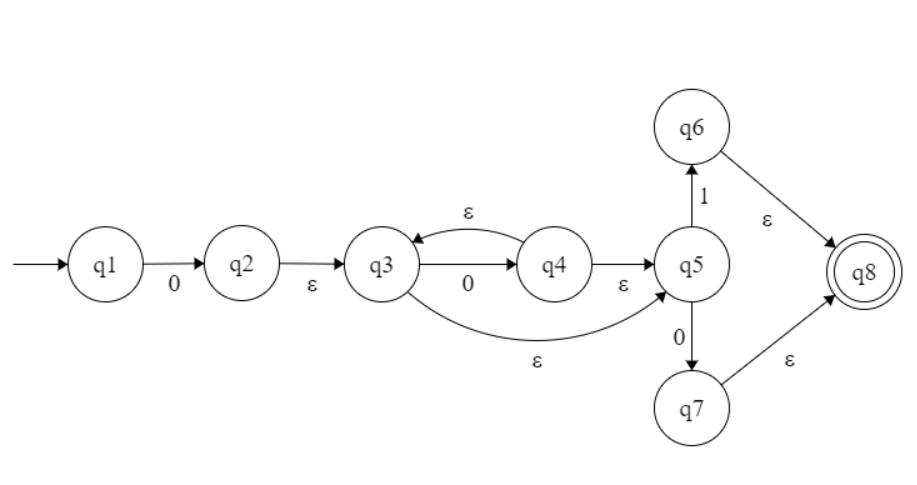
\includegraphics[scale=0.9]{mynd}

\section*{2.}

$(0^{*}1((10^{*}1)\cup(01^{*}0))1)^{*}\cup0^{*}$

\section*{3.}

\subsection*{a)}

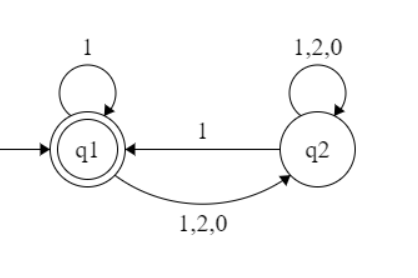
\includegraphics[scale=0.9]{myndb}

\subsection*{b)}

$(1^{*} (1 \cup 2 \cup 0 ) (1 \cup 2 \cup 0 )^{*}1)\cup 1^{*}$

\section*{4.}

\subsection*{a)}

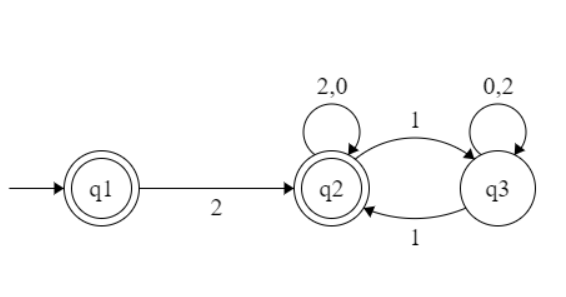
\includegraphics[scale=0.9]{myndc}

\subsection*{b)}

$2((2 \cup 0) \cup (1(0 \cup 2)^{*} 1))^{*}$

\subsection*{c)}

In the input string if there are even numbers of "1" and one or more "2" and any number of "0" then the number is divisible with 2
\end{document}